\begingroup
\def\ThisCaption{A permanent reallocation of gross lending towards existing assets. The shift is $x=0.10$ at $t=0$; all other inputs are in Table~\ref{tab:parameters}. Panels (a) and (b) report log price-level differences from the stationary unchanged-allocation baseline. Panel (c) distinguishes gross and stock shares; dots at $t=-1$ show their initial values. Panel (d) decomposes quarterly relative price growth in the strong-response case as $B_t=G_t-D_t$. The 120-quarter horizon displays convergence, not a forecast.}
\ifdefined\SeparateArtwork
\par\addvspace{0.65\baselineskip}\noindent\begin{minipage}{\linewidth}
\captionsetup{type=figure}
\caption{\ThisCaption}
\label{fig:reallocation}
\centering\small\itshape [Figure \thefigure\ near here]\par
\end{minipage}\par\addvspace{0.65\baselineskip}
\else
\begin{figure}[tbp]
\centering
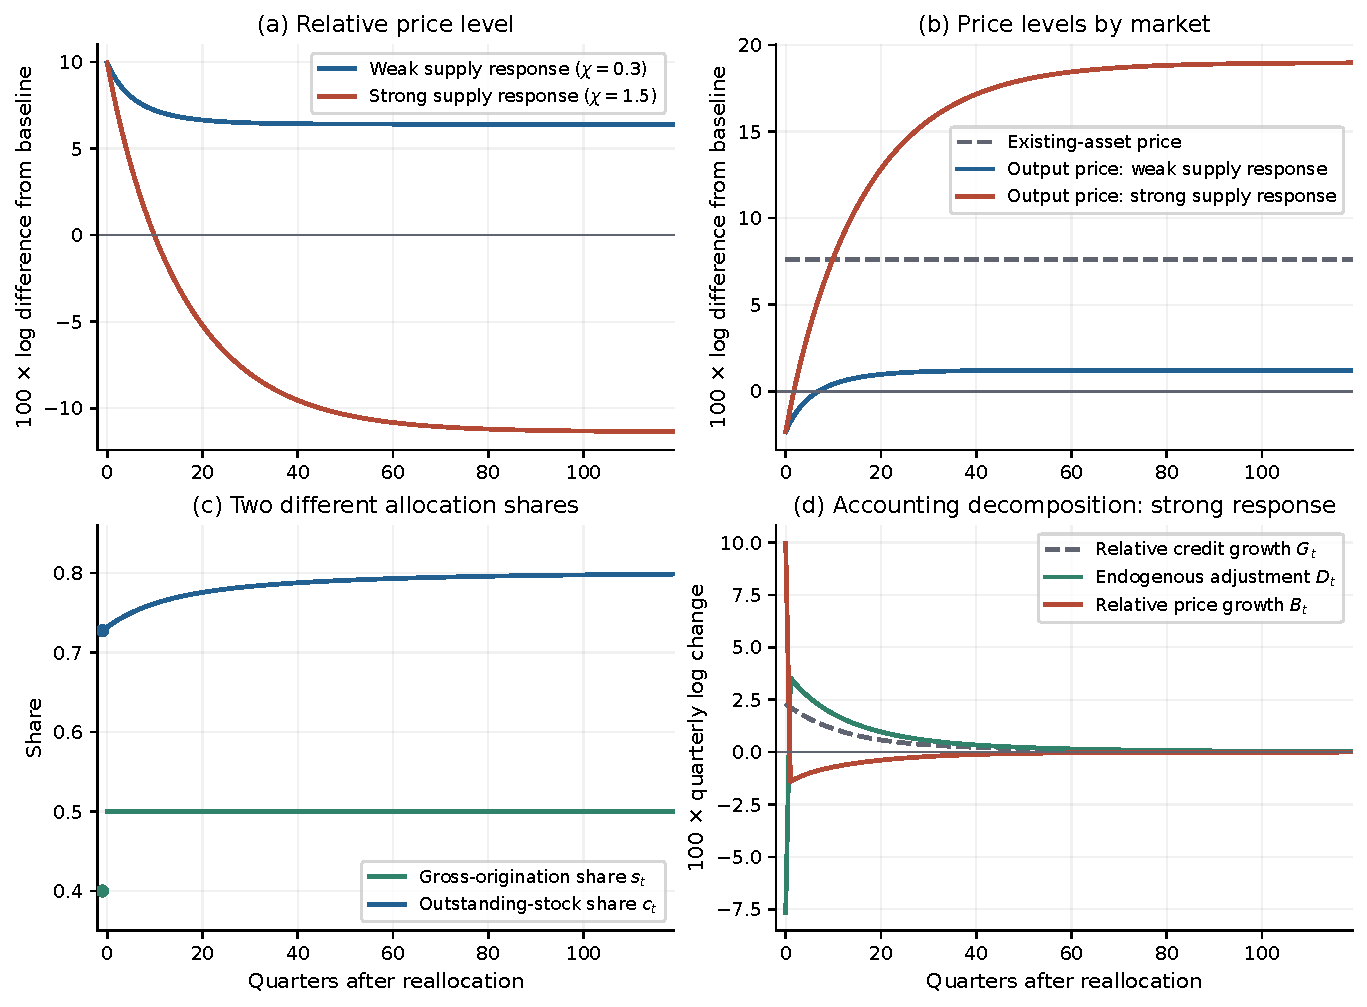
\includegraphics[width=\linewidth]{figures/fig02_reallocation.pdf}
\caption{\ThisCaption}
\label{fig:reallocation}
\end{figure}
\fi
\endgroup
